\begin{frame}
  \frametitle{Organización física de un \textbf{HDD}}
  \begin{figure}
    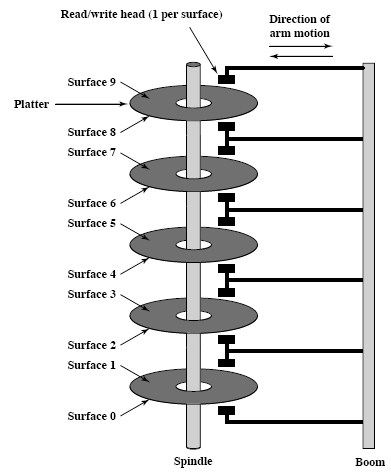
\includegraphics[scale=0.4]{images/disk1.png}
  \end{figure}
\end{frame}

\begin{frame}
  \frametitle{Organización física de un \textbf{HDD} (cont.)}
  \begin{figure}
    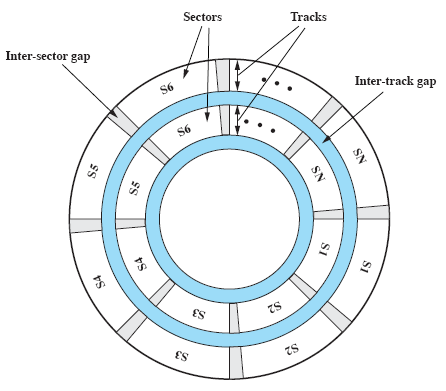
\includegraphics[scale=0.4]{images/disk2.png}
  \end{figure}
\end{frame}

\begin{frame}
  \frametitle{Organización física de un \textbf{HDD} (cont.)}
  \begin{itemize}
  	\item Cilindro N: todas las n-esimas pistas de todas las caras
  \end{itemize}
  \begin{figure}
    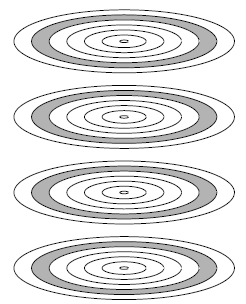
\includegraphics[scale=0.4]{images/cylinders.png}
  \end{figure}
\end{frame}

\begin{frame}
  \frametitle{Capacidad de un disco}
  \begin{itemize}
  	\item La capacidad de un disco esta dada por el producto de:
  	\begin{itemize}
  		\item Cantidad de caras: \emph{W}
  		\item Cantidad de pistas: \emph{X}
  		\item Cantidad de sectores por pista: \emph{Y}
  		\item Tamaño de sector: \emph{Z}
  	\end{itemize}

  	\emph{capadidad = W * X * Y * Z}
  \end{itemize}
\end{frame}

\begin{frame}
  \frametitle{Acceso a un disco}
  \begin{itemize}
  	\item Para realizar una \emph{E/S}, por ejemplo un acceso a disco, se requiere de una llamada al sistema (\textit{System Call}). En la misma se especifica:
  	\begin{itemize}
  		\item Tipo de operación (\emph{E} o \emph{S})
  		\item Dirección en disco para la transferencia (file descriptor que se obtuvo al abrir un archivo)
  		\item Dirección en memoria para la transferencia (de donde se lee o escribe)
  		\item Número de \bytes a transferir
  	\end{itemize}
  	\item Este requerimiento es pasado, por el \textit{kernel}, al subsistema de \emph{E/S} quien lo traduce en: \textbf{(\#Cara, \#Cilindro, \#Sector)}
  \end{itemize}
\end{frame}

\begin{frame}
  \frametitle{Tiempo de acceso a un \textit{HDD}}
  \begin{itemize}
    \item El tiempo de acceso esta dado por:
    \begin{itemize}
      \item \textbf{Seek time} (posicionamiento): tiempo que tarda en posicionarse la cabeza en el cilindro 
      \item \textbf{Latency time} (latencia): tiempo que sucede desde que la cabeza se posiciona en el cilindro hasta que el sector en cuestión pasa por debajo de la misma
      \item \textbf{Transfer time} (transferencia): tiempo de transferencia del sector (bloque) del disco a la memoria
    \end{itemize}    
  \end{itemize}
  \begin{figure}
      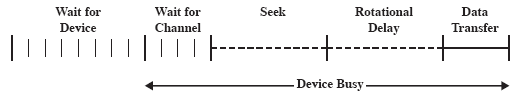
\includegraphics[scale=0.4]{images/dat.png}
  \end{figure}
\end{frame}

\begin{frame}
  \frametitle{Tiempo de acceso a un \textit{HDD} (cont.)}
  \begin{figure}
      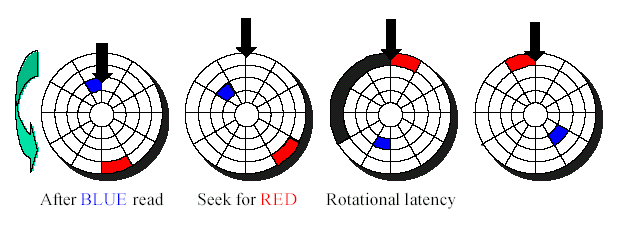
\includegraphics[scale=0.5]{images/dat2.png}
  \end{figure}
\end{frame}

\begin{frame}
  \frametitle{Tiempo de acceso a un \textit{HDD} (cont.)}
  \begin{itemize}
    \item \emph{Latency time} $\rightarrow$ si este tiempo no se conoce, se considera que es igual a lo que tarda el disco en dar media vuelta
    \item Ejemplo. Disco de 5400 \rpm $\rightarrow$
      \linebreak
      \linebreak
      \hspace{35pt} \textcolor{orange}{\textbf{5400 vueltas $\rightarrow$ 1' = 60'' = 60000 \ms}}
      \linebreak  
      \hspace{35pt} \textcolor{orange}{\textbf{1/2 vuelta $\rightarrow$ x = 5,5 \ms}}
  \end{itemize}
\end{frame}

\begin{frame}
  \frametitle{Tiempo de acceso a un \textit{HDD} (cont.)}
  \begin{itemize}
    \item \textbf{Almacenamiento secuencial}:
      \linebreak
      \hspace{35pt} \emph{seek + latency + (tiempo\_transferencia\_bloque * \#bloques)}
    \item \textbf{Almacenamiento aleatorio}:
      \linebreak
      \hspace{35pt} \emph{(seek + latency + tiempo\_transferencia\_bloque) * \#bloques}      
  \end{itemize}
\end{frame}

\begin{frame}
  \frametitle{Prefijos}
  \begin{itemize}
    \item Prefijos: nos permiten representar números largos de manera más reducida
    \item Prefijos binarios: 
    \begin{itemize}
      \item Nos permiten crear múltiplos binarios (basados en potencias de 2)
      \item Son similares, en concepto, aunque difieren en valor a los prefijos del \emph{Sistema Internacional} (SI) basados en potencias de 10
      \item En la práctica se adopta el sistema de prefijos binarios
    \end{itemize}  
  \end{itemize}
\end{frame}

\begin{frame}
  \frametitle{Prefijos - \textbf{Equivalencias}}
  \begin{figure}
      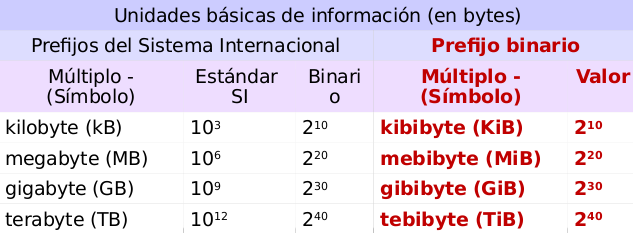
\includegraphics[scale=0.5]{images/si.png}
  \end{figure}
\end{frame}

\begin{frame}
  \frametitle{Capacidad un disco - \textbf{HDD}}
  \begin{itemize}
    \item Supongamos un disco con 6 platos, 2 caras útiles, 1500 pistas por cara y 700 sectores por pista de 256 \bytes cada uno
    \item Si queremos calcular la capacidad total del disco, hacemos:
    \linebreak
    \linebreak
    \emph{tamaño\_disco = \#caras * \#pistas\_cara * \#sectores\_pista * tamaño\_sector}
    \linebreak
    \linebreak
    \textcolor{orange}{\textbf{(6 * 2) * 1500 * 700 * 256 \bytes = 225600000 \bytes = 3,00407 \gibishort\bytesshort (\gibi\bytes)}}
  \end{itemize}
\end{frame}

\begin{frame}
  \frametitle{Ocupación sobre un \textit{HDD} - Ejemplo}
  \begin{itemize}
    \item Supongamos un disco con 6 platos, 2 caras útiles, 1500 pistas por cara y 700 sectores por pista de 256 \bytes cada uno
    \item Si queremos cuantas caras ocupará un archivo de 513 \mebishort\bytes almacenado de manera contigua a partir del primer sector de la primer pista de una cara determinada:
    \begin{itemize}
      \item Calculamos la capacidad de 1 cara:
      \linebreak      
      \hspace{35pt} \textcolor{orange}{\textbf{1500 * 700 * 256 \bytes = 268800000 \bytes}}
      \linebreak
      \item Dividimos el tamaño del archivo por la capacidad de una cara:
      \hspace{35pt} \textcolor{orange}{\textbf{513 \mebishort\bytesshort = 537919488 \bytes}}
      \linebreak
      \hspace{35pt} \textcolor{orange}{\textbf{537919488 / 268800000 = 2,00118  $\rightarrow$ 3 caras}}
    \end{itemize}
  \end{itemize}
\end{frame}

\begin{frame}
  \frametitle{Tiempo de acceso a un \textit{HDD} - Ejemplo}
  \begin{itemize}
    \item Supongamos un disco con 6 platos, 2 caras útiles, 1500 pistas por cara y 700 sectores por pista de 256 \bytes cada uno. El disco gira a 12600 \rpm, tiene un tiempo de posicionamiento (\textit{seek}) de 2 \milisegundos y una velocidad de transferencia de 15 \mebishort\bitsshort/\s (\mebi\bits por \segundo)
    \item Si queremos saber cuantos \milisegundos se tardarían en transferir un archivo \textbf{almacenado de manera contigua y aleatoria} de 4500 sectores
  \end{itemize}
\end{frame}

\begin{frame}
  \frametitle{Tiempo de acceso a un \textit{HDD} - Ejemplo (cont.)}
  \begin{itemize}    
    \item Calculamos los datos que faltan:
    \begin{itemize}
      \item Latencia:
      \linebreak
      \textcolor{orange}{\textbf{12600 vueltas $\rightarrow$ 1\msymbol = 60 \s = 60000 \ms}}
      \linebreak
      \textcolor{orange}{\textbf{0,5 vueltas $\rightarrow$ x = 2,3809 \ms}}
      \linebreak
      \item Transferencia:
      \linebreak
      \textcolor{orange}{\textbf{15 \mebishort\bits $\rightarrow$ 1 \s = 1000 \ms}}
      \linebreak
      \textcolor{orange}{\textbf{256 \bytes $\rightarrow$ x}}
      \linebreak
      \linebreak
      Unificamos unidades:
      \linebreak
      \textcolor{orange}{\textbf{15728640 \bits $\rightarrow$ 1000 \ms}}
      \linebreak
      \textcolor{orange}{\textbf{2048 \bits $\rightarrow$ x = 0,1302 \ms}}
    \end{itemize}
  \end{itemize}
\end{frame}

\begin{frame}
  \frametitle{Tiempo de acceso a un \textit{HDD} - Ejemplo (cont.)}
  \begin{itemize}
    \item Datos obtenidos:
    \begin{itemize}
      \item Seek time: 2 \ms
      \item Latency time: 2,3809 \ms
      \item Tiempo transferencia bloque: 0,1302 \ms
      \item \#bloques: 4500 $\rightarrow$ eventualmente se tienen que calcular
    \end{itemize}
    \item Resultados:
    \begin{itemize}
      \item Almacenamiento secuencial:
      \linebreak
      \textcolor{orange}{\textbf{seek + latency + tiempo\_transferencia\_bloque * \#bloques}}
      \linebreak
      \textcolor{orange}{\textbf{2 + 2,3809 + 0,1302 * 4500 = 590,2809 \ms}}      
      \item Almacenamiento aleatorio:
      \linebreak
      \textcolor{orange}{\textbf{(seek + latency + tiempo\_transferencia\_bloque) * \#bloques}}        
      \linebreak
      \textcolor{orange}{\textbf{(2 + 2,3809 + 0,1302) * 4500 = 20299,95 \ms}}
      \linebreak
    \end{itemize}
  \end{itemize} 
\end{frame}

\begin{frame}
  \frametitle{Planificación de requerimientos de un \textit{HDD}}
  \begin{itemize}
    \item Seek time $\rightarrow$ parámetro que más influye en el tiempo de acceso al disco
    \item El sitema operativo:
    \begin{itemize}
      \item Es responsable de utilizar el hardware en forma eficiente. Para los discos, esto significa obtener el menor tiempo de atención de los requerimientos
      \item Debe por lo tanto minimizar el tiempo de \textit{seek} $\rightarrow$ implica menor distancia de recorrido por el brazo
    \end{itemize}
  \end{itemize}
\end{frame}

\begin{frame}
  \frametitle{Algoritmos de planificación en un \textit{HDD}}
  \begin{itemize}
    \item Objetivo: minimizar el movimiento de la cabeza
    \item Como: ordenando lógicamente los requerimientos pendientes (\emph{que estan en la cola}) al disco, considerando el número de cilindro de cada requerimiento. En cualquier momento se pueden encolar nuevo movimientos
    \item La atención de requerimientos a pistas duplicadas se resuelven según el algoritmo de planificación:
    \begin{itemize}
      \item \textbf{FCFS}: se atienden de manera separada (tantas veces como se requieran). Por ejemplo, si tengo \{10, 40, 70, 10\}, al 10 lo atiendo 2 veces
      \item \textbf{SSTF}/\textbf{SCAN}/\textbf{LOOK}/\textbf{C-SCAN}/\textbf{C-LOOK}: se atienden de manera consecutiva
    \end{itemize}
  \end{itemize}
\end{frame}

\begin{frame}
  \frametitle{Algoritmos - Ejemplo de enunciado sin \textbf{page faults}}
  \begin{itemize}
    \item Cantidad de pistas: 200 (0..199)
    \item Requerimientos en la cola: \{98 , 183 , 37, 122, 14, 124, 65, 67\}
    \item Viene de: pista 61
    \item Ubicación actual del cabezal: pista 53 $\rightarrow$ derecha-izquierda
  \end{itemize}
\end{frame}

\begin{frame}
  \frametitle{\textbf{First Come First Served}}
  \begin{itemize}
    \item \textbf{FCFS}: atiende los requerimientos por orden de llegada
  \end{itemize}
  \begin{figure}
    \includegraphics[scale=0.4]{images/fifo1.png}
  \end{figure}
  \hspace{35pt} \textcolor{orange}{Movimientos: 640}
\end{frame}

\begin{frame}
  \frametitle{\textbf{Sortest Seek Time First}}
  \begin{itemize}
    \item \textbf{SSTF}: selecciona el requerimiento que requiere el menor movimiento del cabezal
  \end{itemize}
  %\begin{figure}
  %  \includegraphics[scale=0.4]{images/sstf1.png}
  %\end{figure}
  \hspace{35pt} \textcolor{orange}{Movimientos: 235}
\end{frame}

\begin{frame}
  \frametitle{\textbf{SCAN}}
  \begin{itemize}
    \item \textbf{SCAN}: barre el disco en una dirección atendiendo los requerimientos pendientes en esa ruta hasta llegar a la última pista y cambia la dirección. Es \textbf{importante} saber en que pista se \textbf{esta} y de que pista se \textbf{viene} para determinar el sentido del cabezal
  \end{itemize}
  %\begin{figure}
  %  \includegraphics[scale=0.4]{images/scan1.png}
  %\end{figure}
  \hspace{35pt} \textcolor{orange}{Movimientos: 236}
\end{frame}

\begin{frame}
  \frametitle{\textbf{LOOK}}
  \begin{itemize}
    \item \textbf{LOOK}: se comporta igual que el \textit{SCAN} pero no llega hasta la última pista del disco sobre la dirección actual sino que llega hasta el último requerimiento de la dirección actual
  \end{itemize}
  %\begin{figure}
  %  \includegraphics[scale=0.4]{images/look1.png}
  %\end{figure}
  \hspace{35pt} \textcolor{orange}{Movimientos: 236}
\end{frame}

\begin{frame}
  \frametitle{\textbf{Circular SCAN}}
  \begin{itemize}
    \item \textbf{C-SCAN}: se comporta igual que el \textit{SCAN} pero restringe la atención en un solo sentido. Al llegar a la última pista del disco en el sentido actual vuelve a la pista del otro extremo (\textbf{salto} $\rightarrow$ no se cuentan los movimientos) y sigue barriendo en el mismo sentido
  \end{itemize}
  %\begin{figure}
  %  \includegraphics[scale=0.4]{images/cscan1.png}
  %\end{figure}
  \hspace{35pt} \textcolor{orange}{Movimientos: 187}
\end{frame}

\begin{frame}
  \frametitle{\textbf{Circular LOOK}}
  \begin{itemize}
    \item \textbf{C-LOOK}: se comporta igual que el \textit{LOOK} pero restringe la atención en un solo sentido. Al llegar a la  última pista de los requerimientos en el sentido actual vuelve a la primer pista más lejana del otro extremo (\textbf{salto} $\rightarrow$ no se cuentan los movimientos) y sigue barriendo en el mismo sentido
  \end{itemize}
  %\begin{figure}
  %  \includegraphics[scale=0.4]{images/clook1.png}
  %\end{figure}
  \hspace{35pt} \textcolor{orange}{Movimientos: 157}
\end{frame}

\begin{frame}
  \frametitle{Algoritmos - Atención de \textbf{PF}}
  \begin{itemize}
    \item Existen requerimientos especiales que deben atenderse con urgencia. Los \textit{fallos de página} indican simplemente que tienen mayor prioridad con respecto a los requerimientos convencionales, por lo tanto deben ser atendidos inmediatamente después del requerimiento que se esta atendiendo actualmente    
    \item La lógica de atención de múltiples \textit{PF} se maneja según el algoritmo de planificación. Ejemplos:
    \begin{itemize}
      \item \textbf{FCFS}: Si tengo \{10, 40PF, 70PF, 10\}, primero se atiende al 40PF y luego al 70PF
      \item \textbf{SSTF}: si tengo \{10, 40PF, 70PF, 10\} y estoy en la pista 65, primero atiendo al 70PF y luego al 40PF
    \end{itemize}
    \item En todos los algoritmos, los movimientos utilizados para atender estos requerimientos especiales deben ser contados
  \end{itemize}
\end{frame}

\begin{frame}
  \frametitle{Algoritmos - Atención de \textbf{PF (cont.)}}
  \begin{itemize}
    \item Una vez que no existan más requerimientos por \textit{page faults} en la cola, se procede:
    \begin{itemize}
      \item \textbf{FCFS}: en orden \textit{FCFS}
      \item \textbf{SSTF}: en orden \textit{SSTF}
      \item \textbf{SCAN}: con el sentido que determina la atención de los últimos dos requerimientos $\rightarrow$ puede cambiar de sentido
      \item \textbf{C-SCAN}: con el sentido original $\rightarrow$ el sentido no cambia
      \item \textbf{LOOK}: del mismo modo en que lo hace el \textit{SCAN}
      \item \textbf{C-LOOK}: del mismo modo en que lo hace el \textit{C-SCAN}
    \end{itemize}
  \end{itemize}
\end{frame}

\begin{frame}
  \frametitle{Algoritmos - Ejemplo de enunciado con \textbf{page faults}}
  \begin{itemize}
    \item Cantidad de pistas: 100 (0..99)
    \item Requerimientos en la cola: \{55 , 75 , \textcolor{red}{25$^{PF}$}, 45, 10\}. Luego de 30 movimientos \{\textcolor{red}{52$^{PF}$}, 60\} y luego de 10 movimientos más (40 desde el comienzo de la planificación) entra \{90, 10\}
    \item Se se viene de la pista 15
    \item Se esta atendiendo la pista 20 $\rightarrow$ izquierda-derecha
  \end{itemize}
\end{frame}

\begin{frame}
  \frametitle{\textbf{First Come First Served}}
  %\begin{figure}
  %  \includegraphics[scale=0.5]{images/fifo2.png}
  %\end{figure}
  \hspace{35pt} \textcolor{orange}{Movimientos: ¿TODO?}
\end{frame}

\begin{frame}
  \frametitle{\textbf{Sortest Seek Time First}}
  %\begin{figure}
  %  \includegraphics[scale=0.5]{images/sstf2.png}
  %\end{figure}
  \hspace{35pt} \textcolor{orange}{Movimientos: 180}
\end{frame}

\begin{frame}
  \frametitle{\textbf{SCAN}}
  %\begin{figure}
  %  \includegraphics[scale=0.5]{images/scan2.png}
  %\end{figure}
  \hspace{35pt} \textcolor{orange}{Movimientos: ¿TODO?}
\end{frame}

\begin{frame}
  \frametitle{\textbf{LOOK}}
  %\begin{figure}
  %  \includegraphics[scale=0.5]{images/look2.png}
  %\end{figure}
  \hspace{35pt} \textcolor{orange}{Movimientos: ¿TODO?}
\end{frame}

\begin{frame}
  \frametitle{\textbf{Circular SCAN}}
  %\begin{figure}
  %  \includegraphics[scale=0.5]{images/cscan2.png}
  %\end{figure}
  \hspace{35pt} \textcolor{orange}{Movimientos: ¿TODO?}
\end{frame}

\begin{frame}
  \frametitle{\textbf{Circular LOOK}}
  %\begin{figure}
  %  \includegraphics[scale=0.5]{images/clook2.png}
  %\end{figure}
  \hspace{35pt} \textcolor{orange}{Movimientos: ¿TODO?}
\end{frame}

%%%%%%%%%%%%%%%%%%%%%%%%%%%%%%%%%%%%%%%%%%%%%%%%%%%%%%%%%%%%%%%%%%

\begin{comment}

\begin{frame}[fragile]
  \frametitle{Características - Configuración de discos (cont.)}
  \begin{itemize}
	  \item A futuro, todos los dispositivos llamados hdX serán denominados sdX $\leftarrow$ Introducido en Debian/Squeeze
	  \item Por estas y otras razones se adoptan 4 mecanismos nuevos para nomenclar\footnote{\url{http://wiki.debian.org/Part-UUID}}:
	  \begin{itemize}
	  	\item Nombres persistentes por \textbf{UUID} (\small{Universal Unique Identifier}):
	  	\begin{lstlisting}
$ ls –l /dev/disk/by-uuid/
2d781b26-0285-421a-b9d0-d4a0d3b55680 -> ../../sda1
31f8eb0d-612b-4805-835e-0e6d8b8c5591 -> ../../sda7
		\end{lstlisting}
		\item Utilizando \textbf{labels}
		\begin{lstlisting}
$ ls -l /dev/disk/by-label
data -> ../../sdb2
data2 -> ../../sda2
		\end{lstlisting}
	  \end{itemize}
  \end{itemize}
\end{frame}

\begin{frame}
  \frametitle{Herramientas para particionar}
  \begin{itemize}
	  \item El particionado de un disco se lo puede realizar mediante:
	  \begin{itemize}
	  	\item Software destructivo: \textit{fdisk}
	  	\item Software no destructivo: \textit{fips}, \textit{gparted}
		\begin{figure}
		    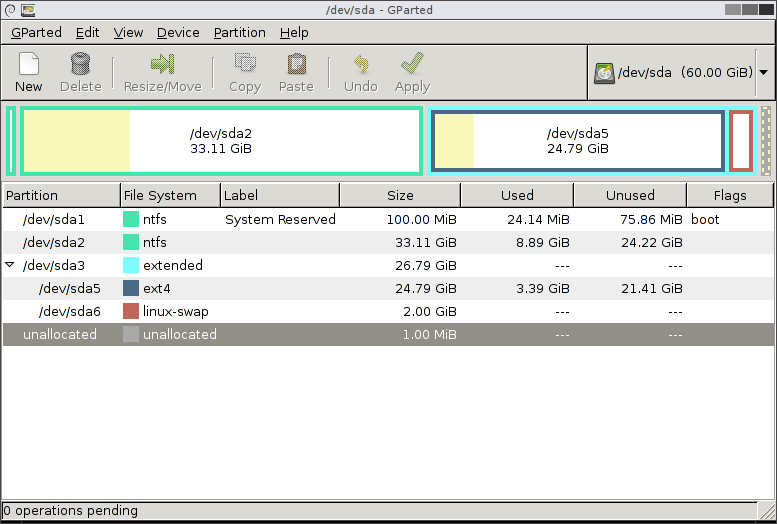
\includegraphics[scale=0.3]{images/gparted.png}
		\end{figure}
	  \end{itemize}
  \end{itemize}
\end{frame}

\begin{frame}[fragile]
  \frametitle{Permisos}
  \begin{itemize}
	  	\item Se aplican a directorios y archivos
	  	\item Existen 3 tipos de permisos y se basan en una notación octal:
	  	\begin{table}
		      \centering
		      \resizebox{10pc}{!}{
			  \begin{tabular}{| c | c | c |}
			      \hline
			      \bf Permiso & \bf Valor & \bf Octal \\
			      \hline
			      Lectura & R & 4 \\
			      \hline
			      Escritura & W & 2 \\
			      \hline
			      Ejecución & X & 1 \\
			      \hline
			  \end{tabular}
		      }
		\end{table}
		\item Se aplican sobre los usuarios:
		\begin{itemize}
			\item Usuario: permisos del dueño $\rightarrow$ \textbf{U}
			\item Usuario: permisos del grupo $\rightarrow$ \textbf{G}
			\item Usuario: permisos de otros usuario $\rightarrow$ \textbf{O}
		\end{itemize}
		\item Se utiliza el comando \textbf{chmod}:
		\begin{lstlisting}
$ chmod 755 /tmp/script
		\end{lstlisting}
  \end{itemize}
\end{frame}
\end{comment}